\documentclass[12pt,letterpaper]{article}
\usepackage{graphicx,textcomp}
\usepackage{natbib}
\usepackage{setspace}
\usepackage{fullpage}
\usepackage{color}
\usepackage[reqno]{amsmath}
\usepackage{amsthm}
\usepackage{amssymb,enumerate}
\usepackage[all]{xy}
\usepackage{endnotes}
\usepackage{lscape}
\newtheorem{com}{Comment}
\newtheorem{lem} {Lemma}
\newtheorem{prop}{Proposition}
\newtheorem{thm}{Theorem}
\newtheorem{defn}{Definition}
\newtheorem{cor}{Corollary}
\newtheorem{obs}{Observation}
\usepackage[compact]{titlesec}
\usepackage{dcolumn}
\usepackage{tikz}
\usetikzlibrary{arrows}
\usepackage{multirow}
\usepackage{xcolor}
\newcolumntype{.}{D{.}{.}{-1}}
\newcolumntype{d}[1]{D{.}{.}{#1}}
\definecolor{light-gray}{gray}{0.65}
\usepackage{url}
\newcommand{\Sref}[1]{Section~\ref{#1}}
\newtheorem{hyp}{Hypothesis}

\title{Machine Learning: Homework 1}
\date{Assigned 1/8, Due 1/15}

\begin{document}
\maketitle


In this homework assignment we're going to analyze the first presidential debate from the 2012 election and then assess the similarity of the statements  \\

We recommend you use the code on the following page for a reference: 

{\tt http://web.stanford.edu/~zlotnick/teaching.html}

In particular, consult the web scraping with BeautifulSoup for details about scraping. 


\section*{Problem 1}
To analyze the debate, we first need to load the debate and parse the content.  On the course {\tt github}, you'll find the file {\tt debate1.html}.  Download the file and open it in a browser. We will use {\tt BeautifulSoup} to parse the HTML file containing the debate transcript.

\begin{itemize}
\item[1)] Load the webpage into {\tt Python} and use {\tt BeautifulSoup} to create a searchable version of the debate. What {\tt HTML} tags can you use to identify statements?

\item[2)] Note that not all of the statements contain information about the speaker. Devise a rule to assign the unlabeled statements to speakers.

\item[] For substantive reasons, we would like to define a single statement as any \textit{uninterrupted} speech from a candidate. We'll say a candidate is interrupted when the transcript says that a new speaker has begun.  In other words, cross talk doesn't count as an interruption. 
\item[3)] With this rule in mind, create a nested {\tt list}.  The outer list will have an entry for each statement.  Each statement will have its own list where the (1) the speaker is identified and (2) the text (and not the tags) of the statment is stored. Remember, some statements are split among several tags; these will need to be concatenated according to the rule you devised above. Remember to filter out notes about audience behavior. Create a parallel {\tt list} that records the speaker of each statement.  
\item Now, we're going to create a document term matrix.  

\begin{itemize}
	\item[i)] For each statement assign it a unique number (place in debate)
	\item[ii)] For each statement identify the speaker (e.g. candidate speaking)
	\item[iii)] Next, we will find the 1000 most used unigrams and the 500 most used trigrams, after removing/simplifying a set of words
\begin{itemize}
	\item[a)] discard punctuation, capitalization, and use {\tt word\_tokenize} to split the text on white space
	\item[b)] Apply the Porter Stemmer to the tokenized documents.  
	\item[c)] Use the stop words from \\
{\tt `http://www.ai.mit.edu/projects/jmlr/papers/volume5/lewis04a/a11-smart-stop-list/english.stop'}
Apply the Porter Stemmer to this list of stop words and discard all stemmed stop words from the speeches. 
\item[d)] Form the list of trigrams using the {\tt trigrams} function from {\tt NLTK}
\item[e)] Use a python dictionary to count the number of times each unigram is used and a second dictionary to count the number of times each trigram is used. These should be counts over the \textit{whole corpus} (that is, all statements).
\end{itemize}

\item[iv)] Write a document-term matrix, where each row contains \\
{\tt Statement \#, Speaker, Uni\_Count$_1$, Uni\_Count$_2$, $\hdots$, Uni\_Count$_{\text{un\_count}}$, Tri\_Count$_1$, Tri\_Count$_2$, $\hdots$, Tri\_Count$_{{\text{tri\_count}}}$ }\\

Remember, if {\tt foo} is a list, you can count the number of times {\tt x} occurs with \\
{\tt foo.count(x)}

\item[v)] Write the document term matrix to a csv file.  Remember that you'll need to reformat the trigram {\tt tuples} so that you don't end up with extra commas in your column names. Use the function from the class notes to take the {\tt tuple}, like \\
{\tt `wabash', `college', `best'} \\
and converts it to\\
{\tt wabash.college.best}
\end{itemize}
\end{itemize}


\section*{Analyzing Document Similarity}

Using the document-term matrix, let's compare the statements.
\begin{itemize}
\item[1)] Create the following six square matrices:
\begin{itemize}
\item[i)] Euclidean distance between documents
\item[ii)] Euclidean distance between documents with tf-idf weights
\item[iii)] Cosine similarity between documents
\item[iv)] Cosine similarity between documents with tf-idf weights
\item[v)] Normalize the rows of the document term matrix.  For row $i$, 
\begin{eqnarray}
\boldsymbol{x}_{i}^{*} & = & \frac{\boldsymbol{x}_{i}}{\sum_{j=1}^{500} x_{ij}} \nonumber 
\end{eqnarray}
Then apply the {\tt Gaussian} kernel to the normalized matrices
\item[vi)] Use the same normalization, but now with tf-idf weights.  Apply the Gaussian kernel.   
\end{itemize}
\item[2)] Using the matrices, identify the most similar (smallest distance) and dissimilar (greatest distance) statements.  Read the pairs of statements---do they appear to actually be similar?  Which method appears to perform best?
\item[3)] Using cosine similarity, compare the average similarity of statements within and between candidates.  Report the results in a table.  
\end{itemize}









\section*{Bonus Question}


\subsubsection*{Problem 3: Probit Regression with a Prior}

Suppose that we assume the following data generation process
\begin{eqnarray}
Y_{i} & \sim & \text{Bernoulli}(\pi_{i} ) \nonumber \\
\pi_{i} & = & \Phi(\boldsymbol{X}_{i} \boldsymbol{\beta}) \nonumber \\
\beta_{j} & \sim & \text{Normal}(\mu, \sigma^{2}_{j} )\nonumber 
\end{eqnarray}

with $\boldsymbol{X}_{i} = (1, x_{i})$ for all $i$ $(i = 1, \hdots, N)$,  $\boldsymbol{\beta} = (\beta_{1}, \beta_{2})$, and $\Phi(\cdot)$ is the cumulative normal distribution function.  \\

We might equivalently write a directed acyclic graph as, 

\vspace{0.25in}

\begin{large}
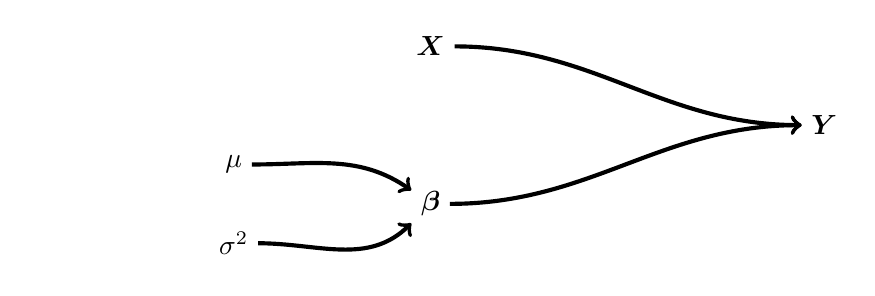
\begin{tikzpicture}
\node(dummy) at (-8, 8) [] {} ; 
\node(covariates) at (-3, 9) [] {$\boldsymbol{X}$} ; 
\node(betas) at (-3, 7) [] {$\boldsymbol{\beta}$ } ; 
\node(prior1) at (-5.5, 7.5) [] {$\mu$ } ; 
\node(prior2) at (-5.5, 6.5) [] {$\sigma^2$ } ; 
\node(dependent) at (2, 8) [] {$\boldsymbol{Y}$};
\draw[->, line width = 1.5pt] (prior1) to [out = 0, in = 145] (betas) ; 
\draw[->, line width = 1.5pt] (prior2) to [out = 0, in = 225] (betas) ; 
\draw[->, line width = 1.5pt] (covariates) to [out = 0, in= 180] (dependent) ; 
\draw[->, line width = 1.5pt] (betas) to [out = 0, in= 180] (dependent) ; 
\end{tikzpicture}
\end{large}


This is very similar to the model described in class, but now we have added a \emph{prior} on $\boldsymbol{\beta}$.  This slightly alters the objective function:

\begin{eqnarray}
p(\boldsymbol{\beta} | \boldsymbol{Y}, \boldsymbol{X}) & \propto & p(\boldsymbol{\beta}|\mu, \sigma^2) \times p(\boldsymbol{Y}| \boldsymbol{X}, \boldsymbol{\beta}) \label{e:post} \\
& \propto &  \prod_{j=1}^{2} \frac{1}{\sqrt{2\pi} \sigma} \exp\left( - \frac{(\beta_{j} - \mu)^2}{2 \sigma^2} \right) \times \prod_{i=1}^{N} \Phi(\boldsymbol{X}_{i}\boldsymbol{\beta})^{Y_{i} } ( 1- \Phi(\boldsymbol{X}_{i}\boldsymbol{\beta})^{1 - Y_{i} } \nonumber 
\end{eqnarray}

In this problem, we will examine how the prior on $\boldsymbol{\beta}$, and in particular the values we set for $\mu$ and $\sigma^2$, alters our inferences about $\boldsymbol{\beta}$.

\begin{itemize}
\item[a)] Analytically, write out the $\log(p(\boldsymbol{\beta} | \boldsymbol{Y}, \boldsymbol{X}))$.  
\item[b)] In {\tt R} create a function for the $\log$ of Equation \ref{e:post}.
\item[c)] Using the synthetic data and the optim guide from class, use {\tt optim} to find $\widehat{\boldsymbol{\beta}}$ with $\mu = 0$ and $\sigma^2 = 1000$
\item[d)] Set $\mu = 1$ and then vary $\sigma^2$.  Using a {\tt for} loop, store estimates of how $\beta_{2}$ changes as you vary $\sigma^2$ from $10$ to $0.01$.  Plot $\beta_{2}$ against $\sigma^2$ and describe what happens as $\sigma^2$ varies.  
\end{itemize}


\end{document}